\documentclass[10pt]{article}
\usepackage[utf8]{inputenc}

\usepackage{geometry}
\usepackage{graphicx}

\geometry{portrait, margin=1.5in}

\begin{document}
\section{Exercise 1 - 20-Time, Reloaded }
The following new classes were created for the implementation of the new wave features.
In the table the responsibilities and collaborations are presented for every class.
\begin{center}
    \begin{tabular}{ | p{3cm} | p{4cm} | p{3cm} | p{2cm} | p{3cm} |}
  \hline
    Class & Responsibility & Collaborates with & Super & Sub \\ \hline
   AlienWaveFactory &Creates alienWave & alienWaveReader, alienWave &  & \\ \hline
   AlienWaveReader & Creates alienWave patterns from file & AlienWavePattern &  & \\ \hline
   AlienWavePattern & Remember pattern of alienWave &  &  &  \\ \hline
   AlienWave &  Data about alienWave & Alien, AlienController  &  & \\ \hline

    \end{tabular}
\end{center}

\subsection{Wave Functional Requirements}

A list of functional requirements considered for the implementation of different waves using the MoSCoW method described in the previous section.

\subsubsection{Must Haves}
The Waves must meet the following requirements:
\begin{itemize}
	\item A new wave shall have a different pattern of aliens.
	\item A wave pattern shall be stored in a file.
	\item Patterns shall be loaded upon starting the game.
\end{itemize}

\subsubsection{Should Haves}
The Waves should meet the following requirements:
\begin{itemize}
	\item Aliens shall have different sizes.
	\item Aliens shall have different types.
	\item The game shall start with a standard pattern. 
	\item The game shall load a random pattern upon loading a wave.
	\item Alien types shall have different colors.
	\item Alien types shall have different shooting speeds.
\end{itemize}

\subsubsection{Could Haves}
The Waves could meet the following requirements:
\begin{itemize}
	\item Different alien types shall take more hits before they die.
	\item Rows of aliens shall move in independent directions of each other.
\end{itemize}
\subsubsection{Would/Won't Haves}
The Waves won't meet the following requirements:
\begin{itemize}
	\item Aliens shall have different movement speeds.
\end{itemize}
\newpage
\subsection{Wave UML}
\begin{figure}[ht!]
\centering
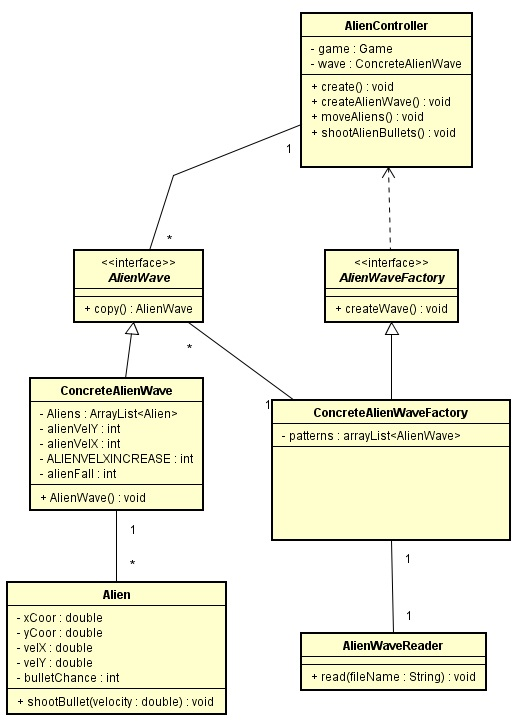
\includegraphics[width=14cm]{waveUML.jpg}
\caption{Wave UML Class Diagram}
\end{figure}
\end{document}
